\documentclass{beamer}
\usepackage[italian]{babel}
\usepackage[T1]{fontenc}
\usetheme{Warsaw}
\usepackage[utf8]{inputenc}
\usepackage{listings}
\usepackage{hyperref}
\usepackage{amsfonts}
\usepackage{multicol}
\usepackage[export]{adjustbox}
\usepackage{graphicx, xcolor, amsmath, amssymb, listings, eurosym, textcomp, galois, amsthm, stmaryrd}
\setbeamercolor*{alerted text}{fg=blue!80!black}

\title{DigiNotar - Untrusted CA}
\subtitle{}
\institute{Università degli Studi di Verona
	\begin{figure}[H]
		\centering
		
\includegraphics[scale=0.1]{univr}
	\end{figure} {\fontsize{3mm}{5mm}\selectfont Progetto per il corso di \textit{"Sicurezza delle Reti"}}}
\author{Marco Colognese - VR423791}
\date{\small Dicembre 2018}


\begin{document}

\begin{frame}
	\titlepage
\end{frame}

\begin{frame}
	\frametitle{Introduzione}
	\begin{itemize}
		\item \textit{DigiNotar}
		\begin{itemize}
			\item La \textit{root CA} olandese
		\end{itemize}
		\item L'attacco al \textit{certificate authority}
			\begin{itemize}
				\item La scoperta dell'attacco
				\item Concretizzazione e conseguenze
				\item Le motivazioni
			\end{itemize}
		\item Le reazioni sul web
			\begin{itemize}
				\item Le principali compagnie
				\item Il governo olandese
			\end{itemize}
		\item Il report di \textit{Fox-IT}
		\begin{itemize}
			\item La pubblicazione del rapporto
			\item L'analisi e la ricostruzione
		\end{itemize}
		\item Comodohacker
			\begin{itemize}
				\item La rivendicazione dell'attacco
				\item Il collegamento con l'attacco a \textit{Comodo Group}
			\end{itemize}
		\item Conclusione
	\end{itemize}
\end{frame}

\title{DigiNotar}
\subtitle{}
\institute{}
\author{}
\date{}
\begin{frame}
	\titlepage
\end{frame}
\title{DigiNotar - Untrusted CA}
\author{Marco Colognese - VR423791}

\begin{frame}
\frametitle{DigiNotar}
\framesubtitle{La \textit{root CA} olandese}
\textit{\alert{DigiNotar}} fu una \alert{root certificate authority} olandese, istituita nel 1998 dal notaio D. Batenburg e dall'ente nazionale dei notai.
\begin{itemize}
	\item Offriva consulenze per implementare servizi elettronici nella propria attività; offriva anche \alert{certificati sicuri}.
	\item È stata una \alert{CA \textit{general-purpose}} per diversi anni, prendendo però di mira il mercato di notai e altri professionisti.
	\item Forniva certificati al \alert{governo olandese} per i servizi online.
	\item Venne acquisita dalla compagnia \alert{\textit{Vasco Data Security International}} nel gennaio 2011.
	\item Nonostante il \alert{primo incidente} nei loro sistemi (giugno 2011), i \alert{certificati} di DigiNotar vennero dichiarati tra i \alert{più affidabili}.
\end{itemize}
\begin{figure}[H]
	\centering
	
\includegraphics[scale=0.45]{diginotar}
\end{figure}
	
\end{frame}

\begin{frame}
\frametitle{DigiNotar}
\framesubtitle{Sistemi per la sicurezza interna}
Poiché i CA sono i primi obiettivi di un attaccante, \textit{DigiNotar} era dotata di importanti sistemi per la sicurezza interna:
\begin{itemize}
	\item reti di computer segmentate per limitare i tentativi di accesso;
	\item \alert{\textit{intrusion prevention system}} per monitorare il traffico entrante;
	\item ogni \alert{richiesta} per un \alert{nuovo certificato} doveva essere approvata da due dipendenti \textit{DigiNotar};
	\item per \alert{pubblicare} il \alert{certificato} era necessario inserire una card in un computer tenuto in una stanza altamente sorvegliata;
	\newline
\end{itemize}
Ciò dimostra che \textit{DigiNotar} aveva investito molto nei propri sistemi di sicurezza interna per mantenere una buona reputazione in rete.
\end{frame}


\title{L'attacco al \textit{certificate authority}}
\subtitle{}
\institute{}
\author{}
\begin{frame}
	\titlepage
\end{frame}
\title{DigiNotar - Untrusted CA}
\author{Marco Colognese - VR423791}

\begin{frame}
\frametitle{L'attacco al \textit{certificate authority}}
\framesubtitle{La scoperta dell'attacco}
Il 27 agosto 2011, un \alert{uomo iraniano} (\textit{alibo}), non riuscendo ad \alert{accedere} all'\alert{email}, segnala il problema al \href{https://productforums.google.com/forum/\#!topic/gmail/3J3r2JqFNTw/discussion}{\alert{\textit{Gmail Help Forum}}}.
\begin{itemize}
	\item Il browser \textit{Chrome} mostrava: \alert{Invalid Server Certificate}.
	\item Il problema sembrava scomparire utilizzando una \alert{\textit{VPN}} che ne mascherava la posizione.
	\item Tutto ciò poteva ricondurre ad eventuali azioni prese dal \alert{governo iraniano} o dall'ISP del paese.
	\item Il rischio era quello di un \textit{\alert{MitM attack}}.
\end{itemize}
\begin{multicols}{2}
	\begin{figure}[H]
		\centering
		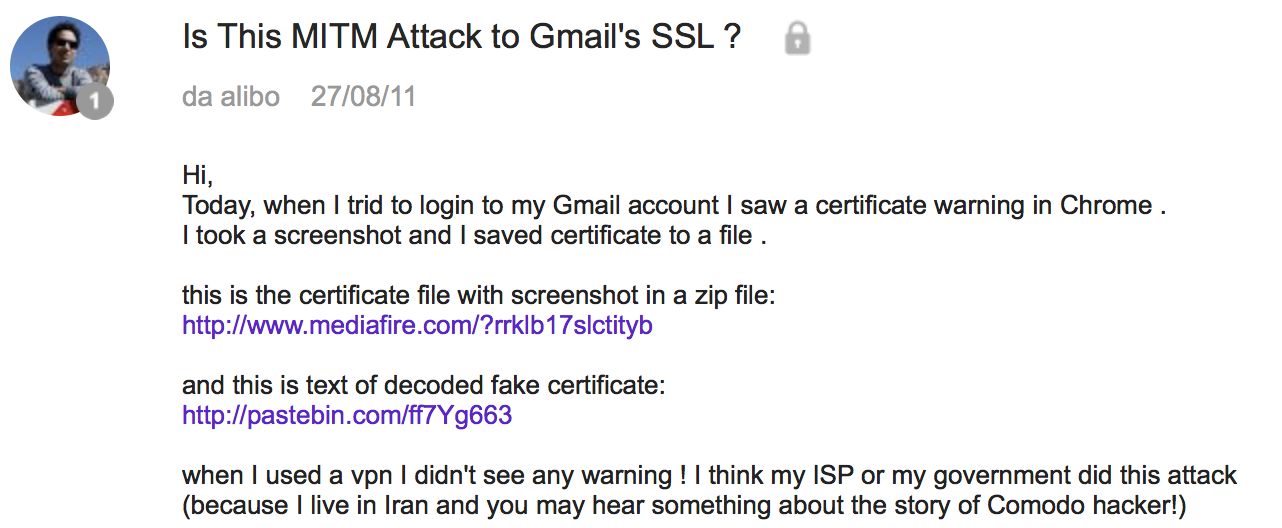
\includegraphics[scale=0.29]{alibo}
	\end{figure}
	\columnbreak
	\begin{figure}[H]
		\centering
		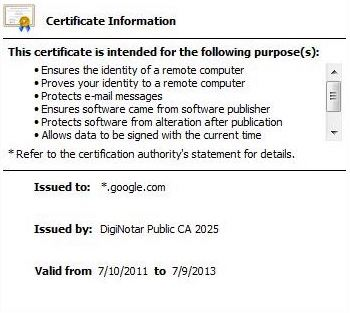
\includegraphics[width=.4\textwidth, right]{invalid}
	\end{figure}
\end{multicols}
\end{frame}


\begin{frame}
\frametitle{L'attacco al \textit{certificate authority}}
\framesubtitle{Concretizzazione}
Nell'\alert{estate del 2011} l'attacco iniziò a concretizzarsi, portando i primi risultati, fino a diventare qualcosa di irreversibile:
\begin{itemize}
	\item Nel mese di giugno un attaccante iniziò a scavare all'interno del labirinto di reti partizionate, fino alla svolta.
	\item Il 10 luglio riesce ad emettere il \alert{primo certificato} compromesso:\\
	\alert{\textit{*.google.com}};
	\item Entro la fine dell'estate si scoprì che furono emessi ben \alert{$531$ certificati} fraudolenti firmati da \textit{DigiNotar}.
	\item Il certificato di \textit{*.google.com} venne individuato da \alert{Chrome} poiché Google, per i propri certificati, riservava \alert{controlli extra}.
\end{itemize}
\begin{figure}[H]
	\centering
	
\includegraphics[scale=0.55]{cert}
\end{figure}
\end{frame}


\begin{frame}
\frametitle{L'attacco al \textit{certificate authority}}
\framesubtitle{Gli errori di \textit{DigiNotar}}
Nonostante \textit{DigiNotar} investisse molto a livello fisico nei propri sistemi di sicurezza, commise importanti \alert{errori a livello software}.
\begin{itemize}
	\item Utilizzava \textit{Windows} e ciascun server si trovava sotto un \alert{unico dominio Windows}; per accedere era sufficiente conoscere la combinazione user/password valida per tutti i server.
	\item La password scelta non era sufficientemente sicura e poteva essere facilmente violata attraverso un \alert{brute-force attack}.
	\item Lasciò in esecuzione nei propri web server alcuni \alert{unpached software}, creando così delle vulnerabilità nel sistema.
	\item Non vi era \alert{nessuna protezione antivirus} all'interno dei server, spianando la strada ad eventuali codici malevoli.
	\item L'\alert{Intrusion Prevention System} era operativo ma \alert{posizionato male} (davanti al firewall), segnalando molti \alert{falsi positivi}.
\end{itemize}
\end{frame}


\begin{frame}
\frametitle{L'attacco al \textit{certificate authority}}
\framesubtitle{La reazione della CA}
Il 19 luglio, un \alert{controllo di routine} rivela l'esistenza di certificati apparentemente firmati da \textit{DigiNotar} che però non erano presenti all'interno dei registri dell'azienda.
\begin{itemize}
	\item questi vengono immediatamente revocati e viene avviata un'indagine interna;
	\item quest'ultima porta alla luce altri \alert{certificati compromessi} che vennero prontamente revocati;
	\item prima della fine di luglio la società \alert{riteneva} che il \alert{problema} fosse definitivamente stato \alert{risolto};
	\item \textit{DigiNotar} scelse di \alert{non comunicare nulla} riguardo l'accaduto, violando il \textit{Dutch Telecommunications Act}.
	\item Fino al 27 agosto, giorno in cui il problema (ancora presente), divenne di dominio pubblico.
\end{itemize}
\end{frame}


\begin{frame}
\frametitle{L'attacco al \textit{certificate authority}}
\framesubtitle{Conseguenze e rischi}
Le \alert{conseguenze} di un attacco di questo genere potevano essere molto gravi. L'emissione di certificati falsi esponeva gli utenti ad attacchi informatici di vario genere:
\begin{itemize}
	\item \alert{Phishing attack}: attraverso un certificato falso l'attaccante può spacciare per sicura una pagina che in realtà è stata creata da lui per estorcere informazioni ad un utente;
	\item  dal precedente si può concretizzare un \alert{MitM attack}, poiché l'attaccante ha il pieno controllo della web page in cui l'utente inserisce i propri dati personali, inconscio del fatto che l'attaccante sta osservando tutto.
	\item la stessa pagina può essere utilizzata per indurre l'utente a scaricare del \alert{codice malevolo} che poi l'attaccante sfrutterà per ottenere un punto di accesso o per altri scopi illeciti.
\end{itemize}

\end{frame}

\begin{frame}
\frametitle{L'attacco al \textit{certificate authority}}
\framesubtitle{Le motivazioni}
I motivi dell'attacco sono stati ricondotti al \alert{governo iraniano} di \textit{Ahmadinejād} che intercettava le comunicazioni della popolazione:
\begin{itemize}
	\item in quel periodo molte persone venivano uccise per aver avuto pareri diversi da chi era al potere;
	\item il governo voleva \alert{controllare} le \alert{email} dei cittadini per individuare i \alert{dissidenti policiti};
	\item questo attacco ha colpito almeno 300 mila persone, di cui il 99\% erano cittadini iraniani;
	\item il sospetto viene quasi confermato dalla "\alert{\textit{firma}}" lasciata dall'\alert{hacker} all'interno di uno \alert{script} in un server;
\end{itemize}
\begin{multicols}{2}
\begin{figure}[H]
	\centering
	
\includegraphics[scale=0.07]{diginotar1}
\end{figure}
\columnbreak
\begin{figure}[H]
	\centering
	
\includegraphics[scale=0.6]{irangmail}
\end{figure}
\end{multicols}
\end{frame}


\title{Le reazioni sul web}
\subtitle{}
\institute{}
\author{}
\begin{frame}
\titlepage
\end{frame}
\title{DigiNotar - Untrusted CA}
\author{Marco Colognese - VR423791}

\begin{frame}
\frametitle{Le reazioni sul web}
\framesubtitle{Le principali compagnie}
Nei giorno 29 e 30 agosto 2011 vengono pubblicati in rete le prime segnalazioni da parte delle compagnie più note:
\begin{itemize}
	\item Nel \textit{\alert{Google Security Blog}} appare un post intitolato:\\ \href{https://security.googleblog.com/2011/08/update-on-attempted-man-in-middle.html}{\textit{"An update on attempted man-in-the-middle attacks"}}.
	\begin{itemize}
		\item Il 3 settembre vengono ufficialmente \alert{respinti} tutti i \alert{certificati} firmati da \textit{DigiNotar}.
	\end{itemize}

	\item Nel \textit{\alert{Mozilla Security Blog}} viene pubblicato un avviso intitolato: \href{https://blog.mozilla.org/security/2011/08/29/fraudulent-google-com-certificate/}{\textit{"Fraudulent *.google.com Certificate"}}.
	\begin{itemize}
		\item Il 2 settembre viene \href{https://blog.mozilla.org/security/2011/09/02/diginotar-removal-follow-up/}{\alert{revocata}} la \alert{fiducia} verso \textit{DigiNotar}, non sapendo quanti altri certificati fraudolenti siano ancora in rete.
	\end{itemize}

	\item \href{https://chromereleases.googleblog.com/2011/08/stable-update.html}{\textit{\alert{Chrome}}} annuncia una nuova release in cui viene \alert{disabilitata} una \alert{\textit{certificate authority}}.
	
	\item Il blog \href{https://blogs.technet.microsoft.com/msrc/2011/08/29/microsoft-releases-security-advisory-2607712/}{\textit{\alert{TechNet}}} di \textit{\alert{Microsoft}} annuncia la rimozione automatica di \textit{DigiNotar} dai CA attendibili da \textit{Windows Vista} e precedenti.
	
\end{itemize}
\noindent
Dopo oltre una settimana di silenzio dalla scoperta, anche \href{https://support.apple.com/it-it/HT4920}{\textit{\alert{Apple}}} annuncia la \alert{rimozione} dei certificati di\textit{DigiNotar} \alert{da Safari}.
\\~\\
\end{frame}

\begin{frame}
\frametitle{Le reazioni sul web}
\framesubtitle{Il governo olandese}
\begin{itemize}
	\item Dopo la scoperta internazionale dell'attacco a \textit{DigiNotar}, il \alert{governo olandese} decise di prendersi a carico la compagnia.
	\item Non ritenevano che i certificati dell'azienda fossero compromessi e continuarono ad utilizzarli per i servizi statali.
	\item Il governo commissionò \alert{Fox-IT} per le indagini sull'accaduto.
	\item Il 3 settembre, dopo i primi risultati dell'indagine, anche il governo passò ad un'altra autorità di certificazione.
	\item Il 20 settembre, \textit{Vasco} annunciò che \textit{DigiNotar} dichiarerà \alert{bancarotta}, presentando un'istanza di fallimento.
\end{itemize}
\begin{figure}[H]
	\centering
	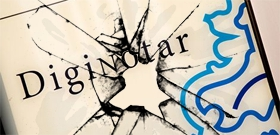
\includegraphics[scale=0.5]{digibreak}
\end{figure}
\end{frame}


\title{Il report di Fox-IT}
\subtitle{}
\institute{}
\author{}
\begin{frame}
	\titlepage
\end{frame}
\title{DigiNotar - Untrusted CA}
\author{Marco Colognese - VR423791}

\begin{frame}
\frametitle{Il report di Fox-IT}
\framesubtitle{La pubblicazione del rapporto}
Il governo olandese aveva incaricato \alert{\textit{Fox-IT}} per effettuare le indagini necessarie e stendere un rapporto dettagliato.

\begin{itemize}
	\item Inizialmente venne chiesto di non pubblicare il rapporto per evitare ulteriori reclami nei confronti di \textit{DigiNotar}.
	\item \alert{Ottobre 2012}: oltre un anno dopo, il \alert{report} dell'operazione \href{https://cryptosense.com/wp-content/uploads/2014/11/black-tulip-update.pdf}{\alert{\textit{Black Tulip}}} viene \alert{pubblicato}.
	\item Si parla di una compromissione quasi totale del sistema.
	\item Identifica la zona con le vittime più colpite (\alert{Iran}), parlando anche di \alert{Comodohacker} ed il suo precedente attacco.
\end{itemize}
	\begin{figure}[H]
		\centering
		
\includegraphics[scale=0.35]{foxit}
	\end{figure}
\end{frame}

\begin{frame}
\frametitle{Il report di Fox-IT}
\framesubtitle{I certificati compromessi}

\begin{minipage}[t]{0.75\textwidth}
	\hspace{0.2cm}
	
	Sono stati identificati $531$ certificati compromessi pubblicati.
	\begin{itemize}
		\item alcuni \alert{certificati non} sono stati \alert{identificati} e potrebbero essere stati utilizzati dallo stato;
		\item l'attacco ha permesso di eseguire \alert{\textit{MitM attack}} in larga scala sugli utenti iraniani di \alert{Gmail}, impersonificando Google in tutti i browser che ritenevano valido il certificato \alert{\textit{*.google.com}} distribuito da \textit{DigiNotar}.
		\item sono stati prodotti certificati anche per altri domini importanti come \alert{Yahoo}, \alert{Mozilla}, \alert{Twitter}, \alert{Microsoft} e \alert{Android}.
	\end{itemize}
\end{minipage}
\begin{minipage}[t]{0.23\textwidth}
	\begin{figure}[H]
		\centering
		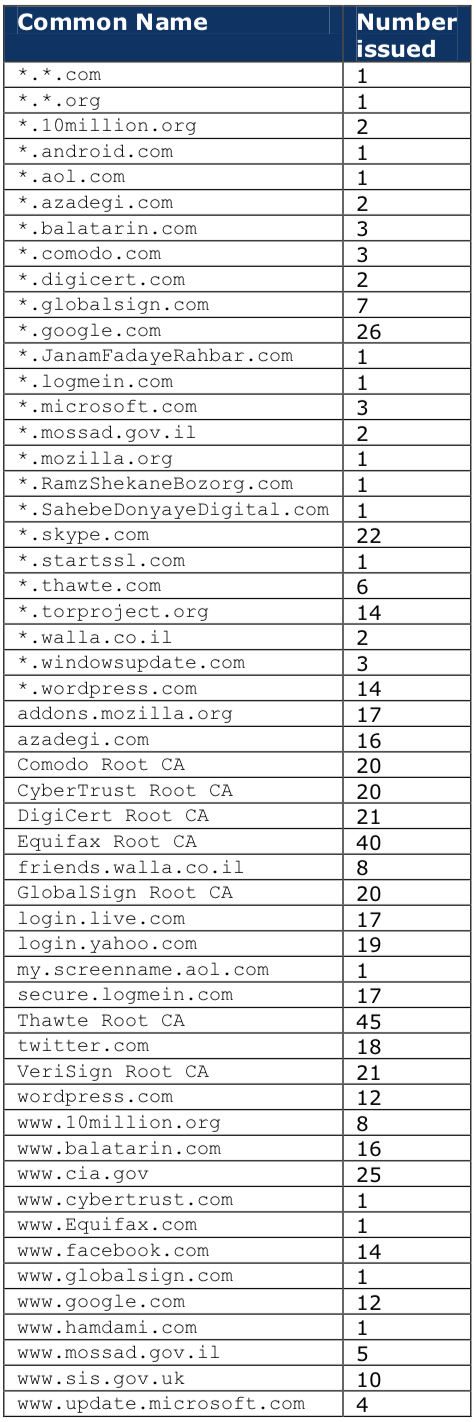
\includegraphics[scale=0.285]{rogue}
	\end{figure}
\end{minipage}
\end{frame}

\begin{frame}
\frametitle{Il report di Fox-IT}
\framesubtitle{L'analisi e la ricostruzione}
\begin{itemize}
	\item L'attaccante aveva il \alert{pieno controllo} di tutti gli 8 \alert{server} della compagnia per la distribuzione di certificati;
	\item I \alert{file di log} per individuare azioni sospette, salvati all'interno dei server compromessi, sono stati anch'essi \alert{manomessi}.
	\item \textit{DigiNotar} possedeva una \alert{rete} interna altamente \alert{segmentata} e separata dall'Internet pubblico.
	\item La società \alert{non aveva} però applicato \alert{regole rigorose} ai \alert{firewall} nella propria rete; ciò avrebbe permesso all'intruso di spostarsi dal web server inizialmente compromesso, al server che ospita le autorità di certificazione.
\end{itemize}
\begin{figure}[H]
	\centering
	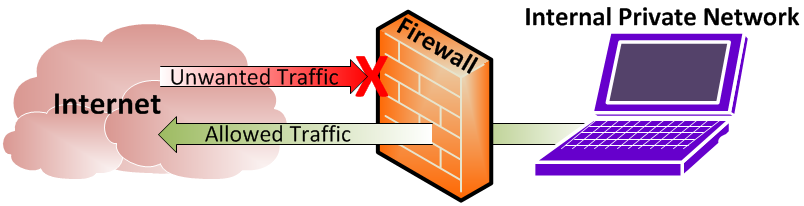
\includegraphics[scale=0.23]{firewall}
\end{figure}
\end{frame}

\begin{frame}
\frametitle{Il report di Fox-IT}
\framesubtitle{L'analisi e la ricostruzione}
\begin{itemize}
	\item L'indagine mostra che i server web nella \alert{zona demilitarizzata esterna} (\textit{DMZ-ext-net}) furono il \alert{primo punto di accesso} per l'intruso il 17 giugno 2011, a causa delle vulnerabilità lasciate dai software non aggiornati.
	\item Tali server venivano usati per \alert{scambiare file} tra sistemi interni ed esterni, con script utili come file manager rudimentali.
	\item Tra il 17 ed il 29 giugno vennero compromessi i sistemi nella \alert{Office-net} e successivamente nella \alert{Secure-net} (1 luglio): la sottorete che ospitava i server della \textit{certificate authority}.
	\item Sono stati recuperati \alert{tool} per \alert{creare tunnel} che permettessero all'attaccante di creare una connessione con i sistemi interni.
	\item Furono recuperati anche \alert{password cracking tool}.
\end{itemize}
\end{frame}

\begin{frame}
\frametitle{Il report di Fox-IT}
\framesubtitle{L'analisi e la ricostruzione}
\begin{itemize}
	\item L'attaccante ha eseguito il tunnelling della connessione \alert{RDP} (\textit{Remote Desktop Protocol}), per ottenere una \alert{GUI} (\textit{Graphical User Interface}) sui sistemi compromessi, inclusi i server CA.
	\item A questo punto l'attaccante aveva il \alert{pieno controllo} della rete, dei server CA, dei file di log e del database.
	\item Per emettere certificati falsi era anche necessario utilizzare una \alert{chiave privata} attiva nel \textit{netHSM (Hardware Security Module)}.
	\item Per attivare le chiavi private sono necessarie delle \alert{smartcard}.
	\item Nei file di log però si trovano voci riguardo la \alert{generazione automatica di CRL} (Certificate Revocation List); le CA le emettono a intervalli regolari secondo le politiche scelte.
\end{itemize}
\end{frame}

\begin{frame}
\frametitle{Il report di Fox-IT}
\framesubtitle{L'analisi e la ricostruzione}
\begin{itemize}
	\item Questi CRL sono firmati dalle autorità emittenti e, per fare ciò, è necessario che la chiave privata sia attiva.
	\item Ciò dimostra che le \alert{chiavi private} erano effettivamente \alert{attive}, offrendo così l'opportunità all'attaccante di produrre e distribuire certificati fraudolenti, identici a quelli affidabili.
	\item Essendo indistinguibili, è necessario \alert{ritirare tutti i certificati} forniti da \textit{DigiNotar} e \alert{rimuovere} la società \alert{dagli elenchi di fiducia} di tutti i software.
\end{itemize}
\begin{figure}[H]
	\centering
	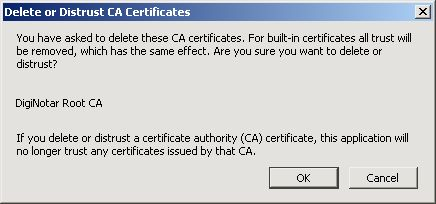
\includegraphics[scale=0.5]{untrust}
\end{figure}
~\\
\end{frame}

\begin{frame}
\frametitle{Il report di Fox-IT}
\framesubtitle{Network security zones}
\begin{figure}[H]
	\centering
	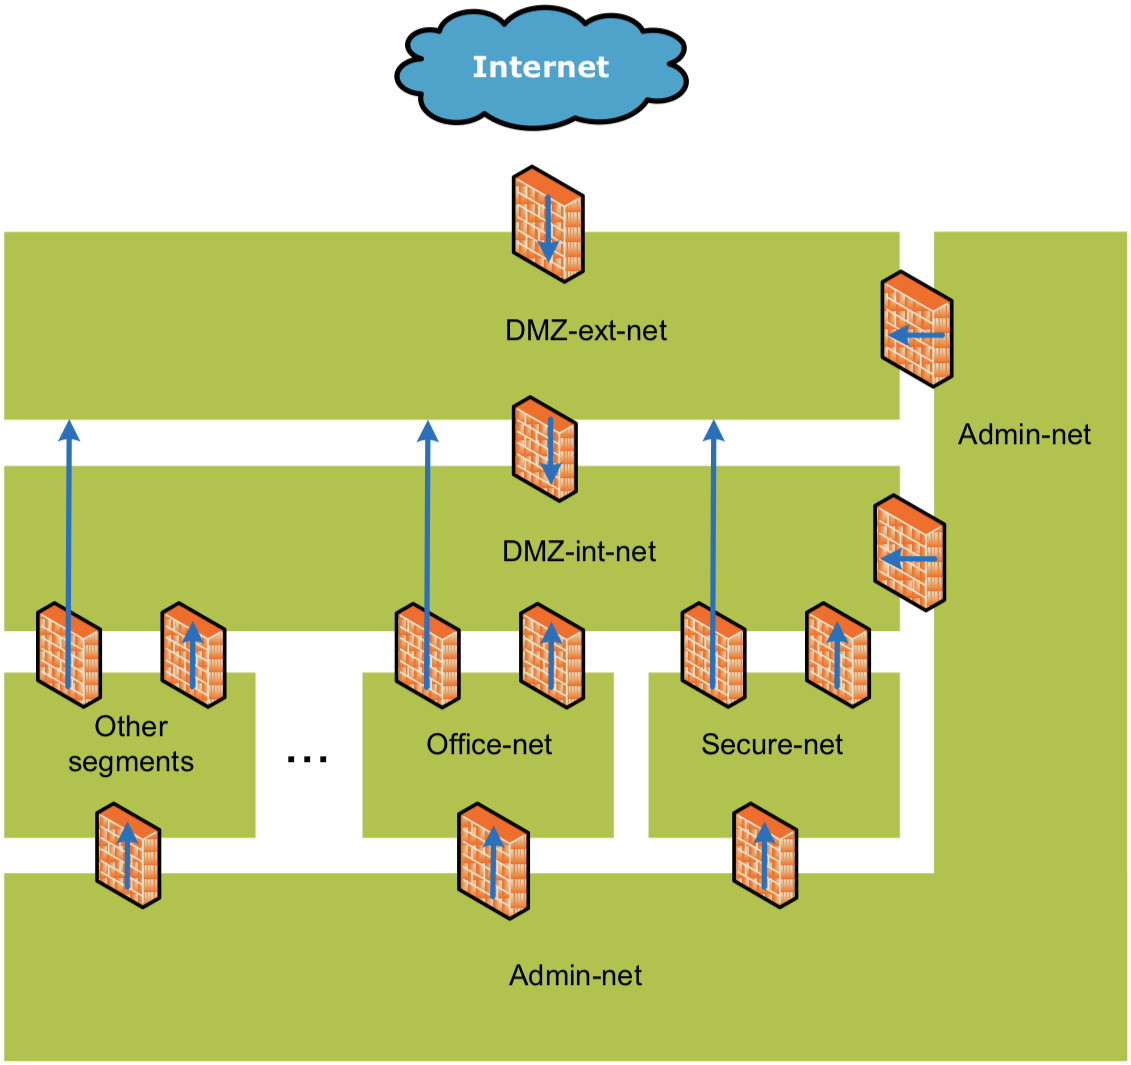
\includegraphics[scale=0.39]{net}
\end{figure}
\end{frame}


\title{ComodoHacker}
\subtitle{}
\institute{}
\author{}
\begin{frame}
	\titlepage
\end{frame}
\title{DigiNotar - Untrusted CA}
\author{Marco Colognese - VR423791}

\begin{frame}
\frametitle{Comodohacker}
\framesubtitle{La rivendicazione dell'attacco}
Il 5 settembre 2011 su \href{https://pastebin.com/1AxH30em}{\textit{\alert{pastebin.com}}} appare un post pubblicato da \textit{\alert{Comodohacker}}, noto da qualche mese per un altro attacco.
\begin{itemize}
	\item Comodohacker si fa chiamare \textit{Ich Sun} ed è un ragazzo 21enne.
	\item È uno \alert{studente iraniano} che sostiene il proprio governo e fa parte di un gruppo di hacker turchi.
	\item Afferma di aver attaccato \textit{DigiNotar} volendo \alert{punire il governo olandese} per le azioni svolte nel 1995 a Srebrenica, con 8000 musulmani uccisi durante la \alert{\textit{Guerra in Bosnia ed Erzegovina}}.
\end{itemize}
Nonostante le dichiarazioni, questa sembra essere soltanto una copertura escogitata dallo stato iraniano per evitare indagini.
\begin{multicols}{2}
\begin{figure}[H]
	\centering
	
\includegraphics[scale=0.35]{iranhack}
\end{figure}
\columnbreak
\begin{figure}[H]
	\centering
	
\includegraphics[scale=0.36]{ira}
\end{figure}
\end{multicols}
\end{frame}


\begin{frame}
\frametitle{Comodohacker}
\framesubtitle{Il collegamento con l'attacco a \textit{Comodo Group}}
Come detto, \textit{Comodohacker} è già noto un altro attacco che prendeva di mira un'altra CA: \textit{Comodo Group}.
\begin{itemize}
	\item Il 15 marzo 2011 era riuscito \alert{compromettere un account} con autorità di registrazione per poter creare un nuovo profilo.
	\item Con il nuovo account ha \alert{creato} e pubblicato 9 \alert{certificati} fraudolenti per 7 domini.
	\item Entro una settimana Comodo ha \alert{ripristinato} la situazione revocando i certificati e incrementando le misure di sicurezza.
	\item L'attacco è stato fatto risalire ad un IP con origine a Teheran in Iran; subito si pensò ad un attacco guidato dallo stato (con il dubbio che l'origine fosse solo un falso indizio).
	\item Il 26 marzo \alert{Comodohacker} rivendica l'attacco su \href{https://pastebin.com/74KXCaEZ}{\alert{\textit{pastebin.com}}}.
\end{itemize}
\begin{figure}[H]
	\centering
	
\includegraphics[scale=0.15]{comodo}
\end{figure}
\end{frame}


\title{Conclusione}
\subtitle{}
\institute{}
\author{}
\begin{frame}
\titlepage
\end{frame}
\title{DigiNotar - Untrusted CA}
\author{Marco Colognese - VR423791}

\begin{frame}
\frametitle{Conclusione}
Il disastro che coinvolse \alert{\textit{DigiNotar}} fu un doloroso campanello d'\alert{allarme per il mondo}, non solo per il governo olandese.
\begin{itemize}
	\item La violazione ha avuto notevoli \alert{ripercussioni} in diverse parti del mondo, in particolare per gli \alert{utenti Gmail} residenti in \alert{Iran}.
	\item Attraverso Internet, le \alert{falle di sicurezza} di un'azienda possono causare \alert{conseguenze terribili} in altre parti del mondo.
	\item Anche le \alert{autorità di certificazione} sulle quali si basa la fiducia mondiale a livello di rete possono essere \alert{vittime di attacchi}.
	\item Non deve essere ammissibile \alert{nessun tipo di negligenza} a livello di sicurezza interna da parte di queste compagnie.
\end{itemize}
\begin{multicols}{2}
\begin{figure}[H]
	\centering
	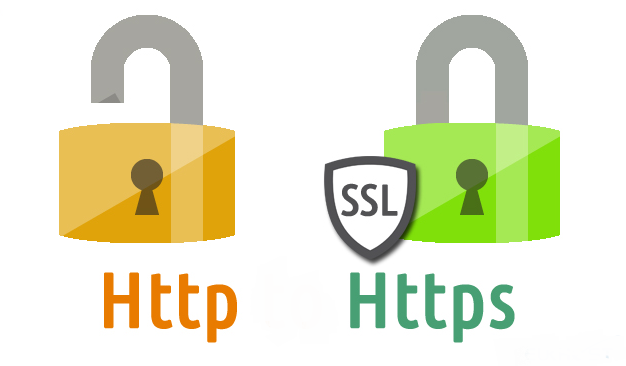
\includegraphics[scale=0.25]{https}
\end{figure}
\columnbreak
\begin{figure}[H]
	\centering
	
\includegraphics[scale=0.35]{secure}
\end{figure}
\end{multicols}
\end{frame}


\end{document}